\documentclass[twoside]{book}

% Packages required by doxygen
\usepackage{fixltx2e}
\usepackage{calc}
\usepackage{doxygen}
\usepackage[export]{adjustbox} % also loads graphicx
\usepackage{graphicx}
\usepackage[utf8]{inputenc}
\usepackage{makeidx}
\usepackage{multicol}
\usepackage{multirow}
\PassOptionsToPackage{warn}{textcomp}
\usepackage{textcomp}
\usepackage[nointegrals]{wasysym}
\usepackage[table]{xcolor}

% Font selection
\usepackage[T1]{fontenc}
\usepackage[scaled=.90]{helvet}
\usepackage{courier}
\usepackage{amssymb}
\usepackage{sectsty}
\renewcommand{\familydefault}{\sfdefault}
\allsectionsfont{%
  \fontseries{bc}\selectfont%
  \color{darkgray}%
}
\renewcommand{\DoxyLabelFont}{%
  \fontseries{bc}\selectfont%
  \color{darkgray}%
}
\newcommand{\+}{\discretionary{\mbox{\scriptsize$\hookleftarrow$}}{}{}}

% Page & text layout
\usepackage{geometry}
\geometry{%
  a4paper,%
  top=2.5cm,%
  bottom=2.5cm,%
  left=2.5cm,%
  right=2.5cm%
}
\tolerance=750
\hfuzz=15pt
\hbadness=750
\setlength{\emergencystretch}{15pt}
\setlength{\parindent}{0cm}
\setlength{\parskip}{0.2cm}
\makeatletter
\renewcommand{\paragraph}{%
  \@startsection{paragraph}{4}{0ex}{-1.0ex}{1.0ex}{%
    \normalfont\normalsize\bfseries\SS@parafont%
  }%
}
\renewcommand{\subparagraph}{%
  \@startsection{subparagraph}{5}{0ex}{-1.0ex}{1.0ex}{%
    \normalfont\normalsize\bfseries\SS@subparafont%
  }%
}
\makeatother

% Headers & footers
\usepackage{fancyhdr}
\pagestyle{fancyplain}
\fancyhead[LE]{\fancyplain{}{\bfseries\thepage}}
\fancyhead[CE]{\fancyplain{}{}}
\fancyhead[RE]{\fancyplain{}{\bfseries\leftmark}}
\fancyhead[LO]{\fancyplain{}{\bfseries\rightmark}}
\fancyhead[CO]{\fancyplain{}{}}
\fancyhead[RO]{\fancyplain{}{\bfseries\thepage}}
\fancyfoot[LE]{\fancyplain{}{}}
\fancyfoot[CE]{\fancyplain{}{}}
\fancyfoot[RE]{\fancyplain{}{\bfseries\scriptsize Generated on Thu Mar 3 2016 10\+:59\+:06 for My Project by Doxygen }}
\fancyfoot[LO]{\fancyplain{}{\bfseries\scriptsize Generated on Thu Mar 3 2016 10\+:59\+:06 for My Project by Doxygen }}
\fancyfoot[CO]{\fancyplain{}{}}
\fancyfoot[RO]{\fancyplain{}{}}
\renewcommand{\footrulewidth}{0.4pt}
\renewcommand{\chaptermark}[1]{%
  \markboth{#1}{}%
}
\renewcommand{\sectionmark}[1]{%
  \markright{\thesection\ #1}%
}

% Indices & bibliography
\usepackage{natbib}
\usepackage[titles]{tocloft}
\setcounter{tocdepth}{3}
\setcounter{secnumdepth}{5}
\makeindex

% Hyperlinks (required, but should be loaded last)
\usepackage{ifpdf}
\ifpdf
  \usepackage[pdftex,pagebackref=true]{hyperref}
\else
  \usepackage[ps2pdf,pagebackref=true]{hyperref}
\fi
\hypersetup{%
  colorlinks=true,%
  linkcolor=blue,%
  citecolor=blue,%
  unicode%
}

% Custom commands
\newcommand{\clearemptydoublepage}{%
  \newpage{\pagestyle{empty}\cleardoublepage}%
}


%===== C O N T E N T S =====

\begin{document}

% Titlepage & ToC
\hypersetup{pageanchor=false,
             bookmarks=true,
             bookmarksnumbered=true,
             pdfencoding=unicode
            }
\pagenumbering{roman}
\begin{titlepage}
\vspace*{7cm}
\begin{center}%
{\Large My Project }\\
\vspace*{1cm}
{\large Generated by Doxygen 1.8.9.1}\\
\vspace*{0.5cm}
{\small Thu Mar 3 2016 10:59:06}\\
\end{center}
\end{titlepage}
\clearemptydoublepage
\tableofcontents
\clearemptydoublepage
\pagenumbering{arabic}
\hypersetup{pageanchor=true}

%--- Begin generated contents ---
\chapter{Hierarchical Index}
\section{Class Hierarchy}
This inheritance list is sorted roughly, but not completely, alphabetically\+:\begin{DoxyCompactList}
\item \contentsline{section}{Makhluk}{\pageref{class_makhluk}}{}
\begin{DoxyCompactList}
\item \contentsline{section}{Hewan}{\pageref{class_hewan}}{}
\begin{DoxyCompactList}
\item \contentsline{section}{Herbivor}{\pageref{class_herbivor}}{}
\begin{DoxyCompactList}
\item \contentsline{section}{Jerapah}{\pageref{class_jerapah}}{}
\item \contentsline{section}{Kuda}{\pageref{class_kuda}}{}
\end{DoxyCompactList}
\item \contentsline{section}{Karnivor}{\pageref{class_karnivor}}{}
\begin{DoxyCompactList}
\item \contentsline{section}{Serigala}{\pageref{class_serigala}}{}
\item \contentsline{section}{Singa}{\pageref{class_singa}}{}
\end{DoxyCompactList}
\end{DoxyCompactList}
\item \contentsline{section}{Tubuhan}{\pageref{class_tubuhan}}{}
\end{DoxyCompactList}
\item Tumbuhan\begin{DoxyCompactList}
\item \contentsline{section}{Rumput}{\pageref{class_rumput}}{}
\item \contentsline{section}{Wortel}{\pageref{class_wortel}}{}
\end{DoxyCompactList}
\end{DoxyCompactList}

\chapter{Class Index}
\section{Class List}
Here are the classes, structs, unions and interfaces with brief descriptions\+:\begin{DoxyCompactList}
\item\contentsline{section}{\hyperlink{class_herbivor}{Herbivor} }{\pageref{class_herbivor}}{}
\item\contentsline{section}{\hyperlink{class_hewan}{Hewan} }{\pageref{class_hewan}}{}
\item\contentsline{section}{\hyperlink{class_jerapah}{Jerapah} }{\pageref{class_jerapah}}{}
\item\contentsline{section}{\hyperlink{class_karnivor}{Karnivor} }{\pageref{class_karnivor}}{}
\item\contentsline{section}{\hyperlink{class_kuda}{Kuda} }{\pageref{class_kuda}}{}
\item\contentsline{section}{\hyperlink{class_makhluk}{Makhluk} }{\pageref{class_makhluk}}{}
\item\contentsline{section}{\hyperlink{class_rumput}{Rumput} }{\pageref{class_rumput}}{}
\item\contentsline{section}{\hyperlink{class_serigala}{Serigala} }{\pageref{class_serigala}}{}
\item\contentsline{section}{\hyperlink{class_singa}{Singa} }{\pageref{class_singa}}{}
\item\contentsline{section}{\hyperlink{class_tubuhan}{Tubuhan} }{\pageref{class_tubuhan}}{}
\item\contentsline{section}{\hyperlink{class_wortel}{Wortel} }{\pageref{class_wortel}}{}
\end{DoxyCompactList}

\chapter{Class Documentation}
\hypertarget{class_herbivor}{}\section{Herbivor Class Reference}
\label{class_herbivor}\index{Herbivor@{Herbivor}}
Inheritance diagram for Herbivor\+:\begin{figure}[H]
\begin{center}
\leavevmode
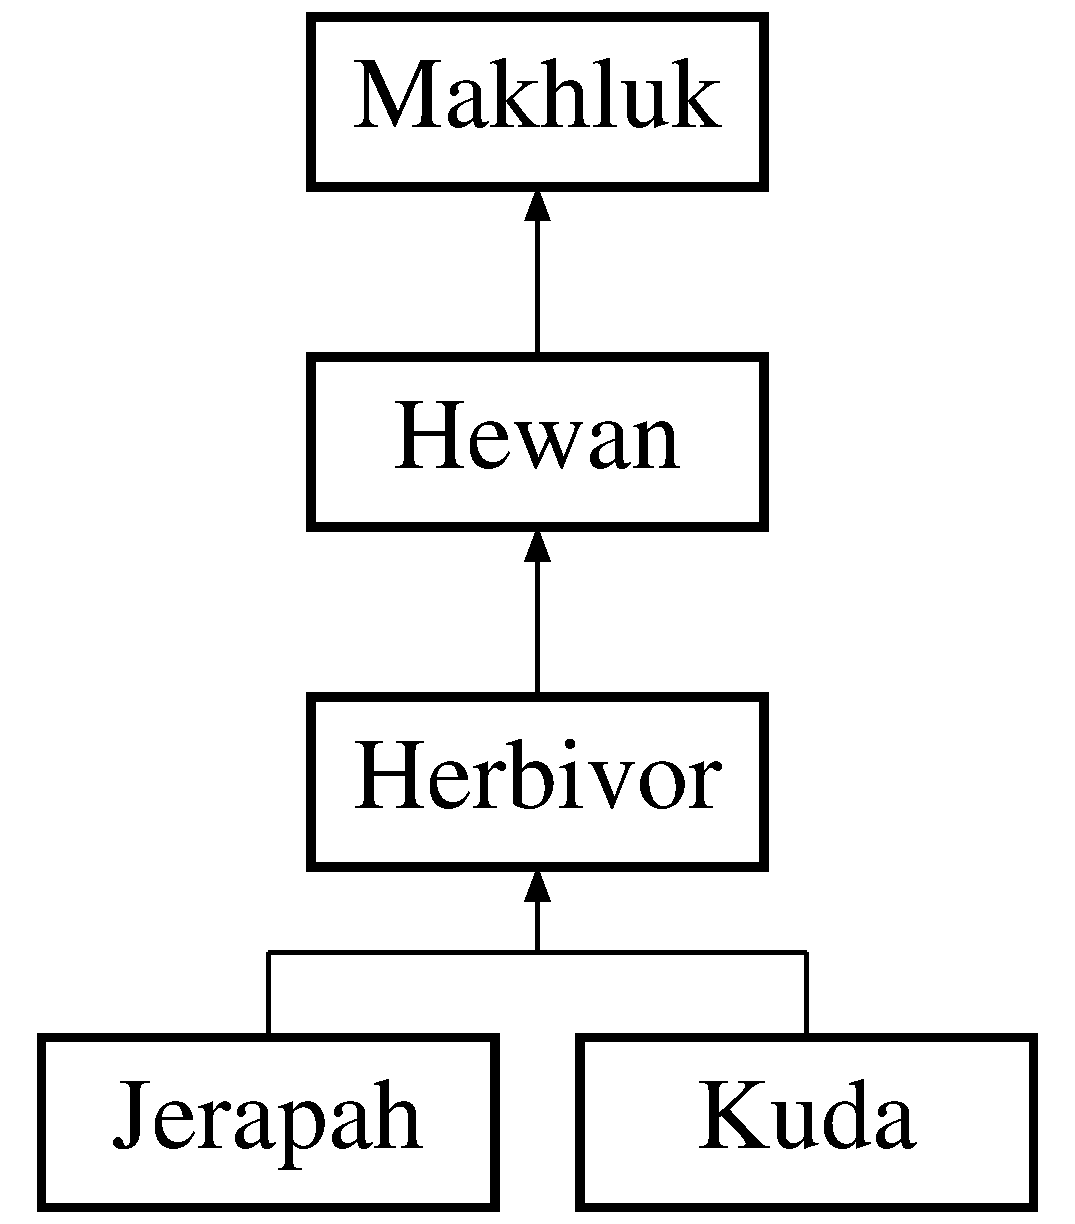
\includegraphics[height=4.000000cm]{class_herbivor}
\end{center}
\end{figure}
\subsection*{Public Member Functions}
\begin{DoxyCompactItemize}
\item 
\hypertarget{class_herbivor_a0566325e084c521e29d3b1ada88db6e8}{}virtual void {\bfseries pass} ()=0\label{class_herbivor_a0566325e084c521e29d3b1ada88db6e8}

\end{DoxyCompactItemize}
\subsection*{Additional Inherited Members}


The documentation for this class was generated from the following file\+:\begin{DoxyCompactItemize}
\item 
src/Herbivor.\+h\end{DoxyCompactItemize}

\hypertarget{class_hewan}{}\section{Hewan Class Reference}
\label{class_hewan}\index{Hewan@{Hewan}}
Inheritance diagram for Hewan\+:\begin{figure}[H]
\begin{center}
\leavevmode
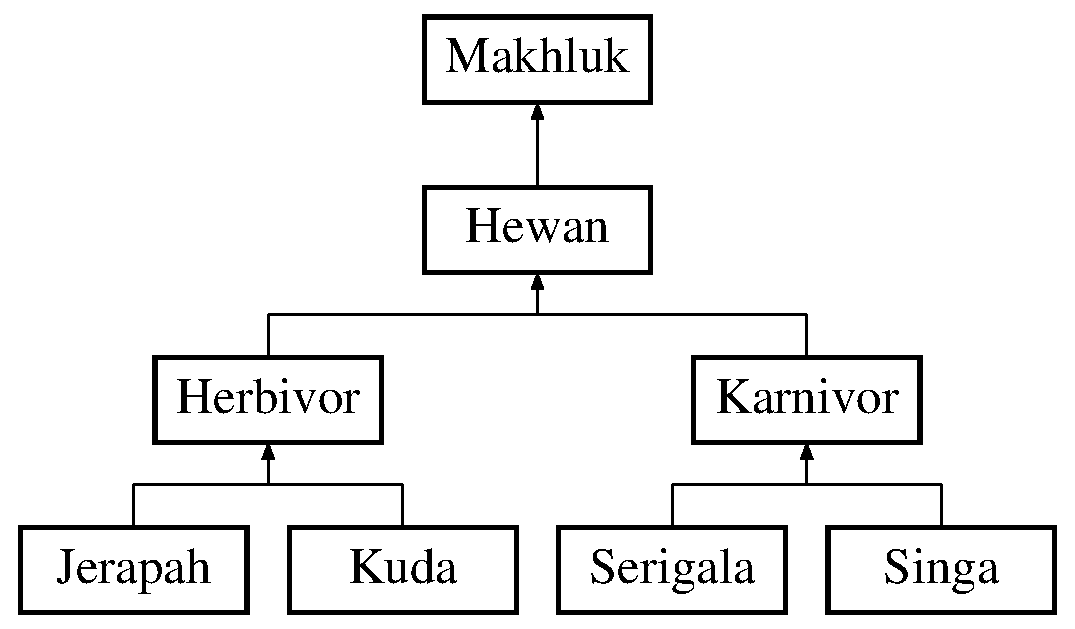
\includegraphics[height=4.000000cm]{class_hewan}
\end{center}
\end{figure}
\subsection*{Public Member Functions}
\begin{DoxyCompactItemize}
\item 
\hypertarget{class_hewan_a8fc5ef4205a20f72339e5576d5bafad5}{}virtual void {\bfseries move} ()=0\label{class_hewan_a8fc5ef4205a20f72339e5576d5bafad5}

\item 
\hypertarget{class_hewan_ab091ad8e469a41a3ad975c93d19c5387}{}virtual void {\bfseries grouping} ()=0\label{class_hewan_ab091ad8e469a41a3ad975c93d19c5387}

\end{DoxyCompactItemize}
\subsection*{Protected Attributes}
\begin{DoxyCompactItemize}
\item 
\hypertarget{class_hewan_ab5383da8d9339d4dfe14a1df5816f8f3}{}int {\bfseries Arah\+Gerak}\label{class_hewan_ab5383da8d9339d4dfe14a1df5816f8f3}

\end{DoxyCompactItemize}


The documentation for this class was generated from the following file\+:\begin{DoxyCompactItemize}
\item 
src/Hewan.\+h\end{DoxyCompactItemize}

\hypertarget{class_jerapah}{}\section{Jerapah Class Reference}
\label{class_jerapah}\index{Jerapah@{Jerapah}}
Inheritance diagram for Jerapah\+:\begin{figure}[H]
\begin{center}
\leavevmode
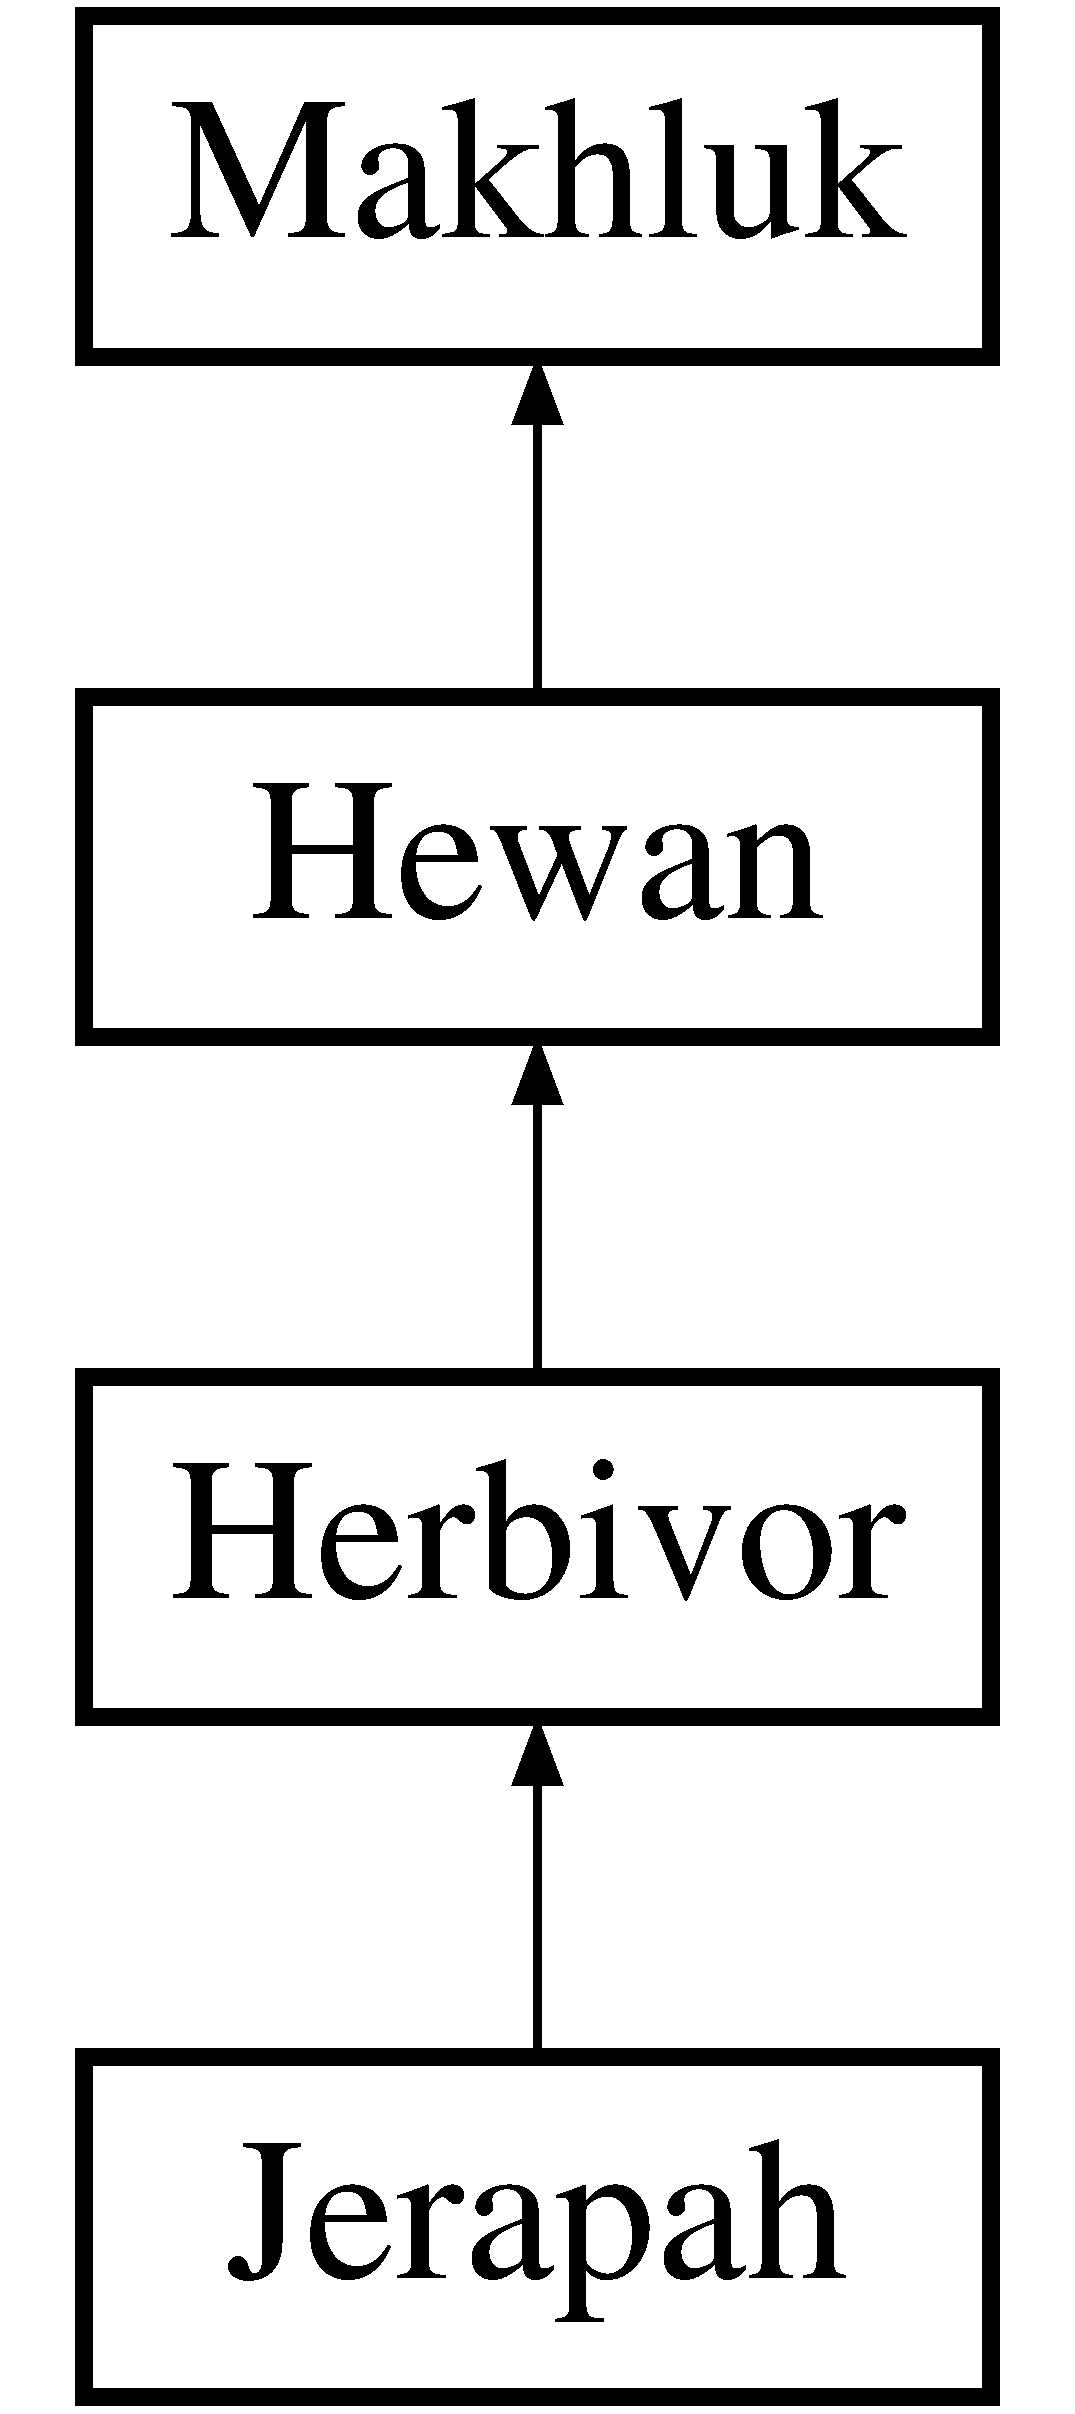
\includegraphics[height=4.000000cm]{class_jerapah}
\end{center}
\end{figure}
\subsection*{Public Member Functions}
\begin{DoxyCompactItemize}
\item 
\hypertarget{class_jerapah_ae137c991cfbc6ff9ebcaa074e5968993}{}{\bfseries Jerapah} (int Power, int Usia, int Posisi\+Awal, int Arah\+Gerak, int Id)\label{class_jerapah_ae137c991cfbc6ff9ebcaa074e5968993}

\item 
\hypertarget{class_jerapah_acb4714a510027900c4a3cb49acbdff5d}{}void {\bfseries Kill} (int id)\label{class_jerapah_acb4714a510027900c4a3cb49acbdff5d}

\item 
\hypertarget{class_jerapah_abb8dd76c0480d03bb6cb8784dce6f6f0}{}void {\bfseries Destruct} ()\label{class_jerapah_abb8dd76c0480d03bb6cb8784dce6f6f0}

\item 
\hypertarget{class_jerapah_a5a1dcc4324ff51a96d1e853d437a3017}{}void {\bfseries Move} ()\label{class_jerapah_a5a1dcc4324ff51a96d1e853d437a3017}

\item 
\hypertarget{class_jerapah_ad8ac2941f6d41b41515ec1ef31cd8556}{}void {\bfseries Pass} ()\label{class_jerapah_ad8ac2941f6d41b41515ec1ef31cd8556}

\end{DoxyCompactItemize}
\subsection*{Additional Inherited Members}


The documentation for this class was generated from the following file\+:\begin{DoxyCompactItemize}
\item 
src/Jerapah.\+h\end{DoxyCompactItemize}

\hypertarget{class_karnivor}{}\section{Karnivor Class Reference}
\label{class_karnivor}\index{Karnivor@{Karnivor}}
Inheritance diagram for Karnivor\+:\begin{figure}[H]
\begin{center}
\leavevmode
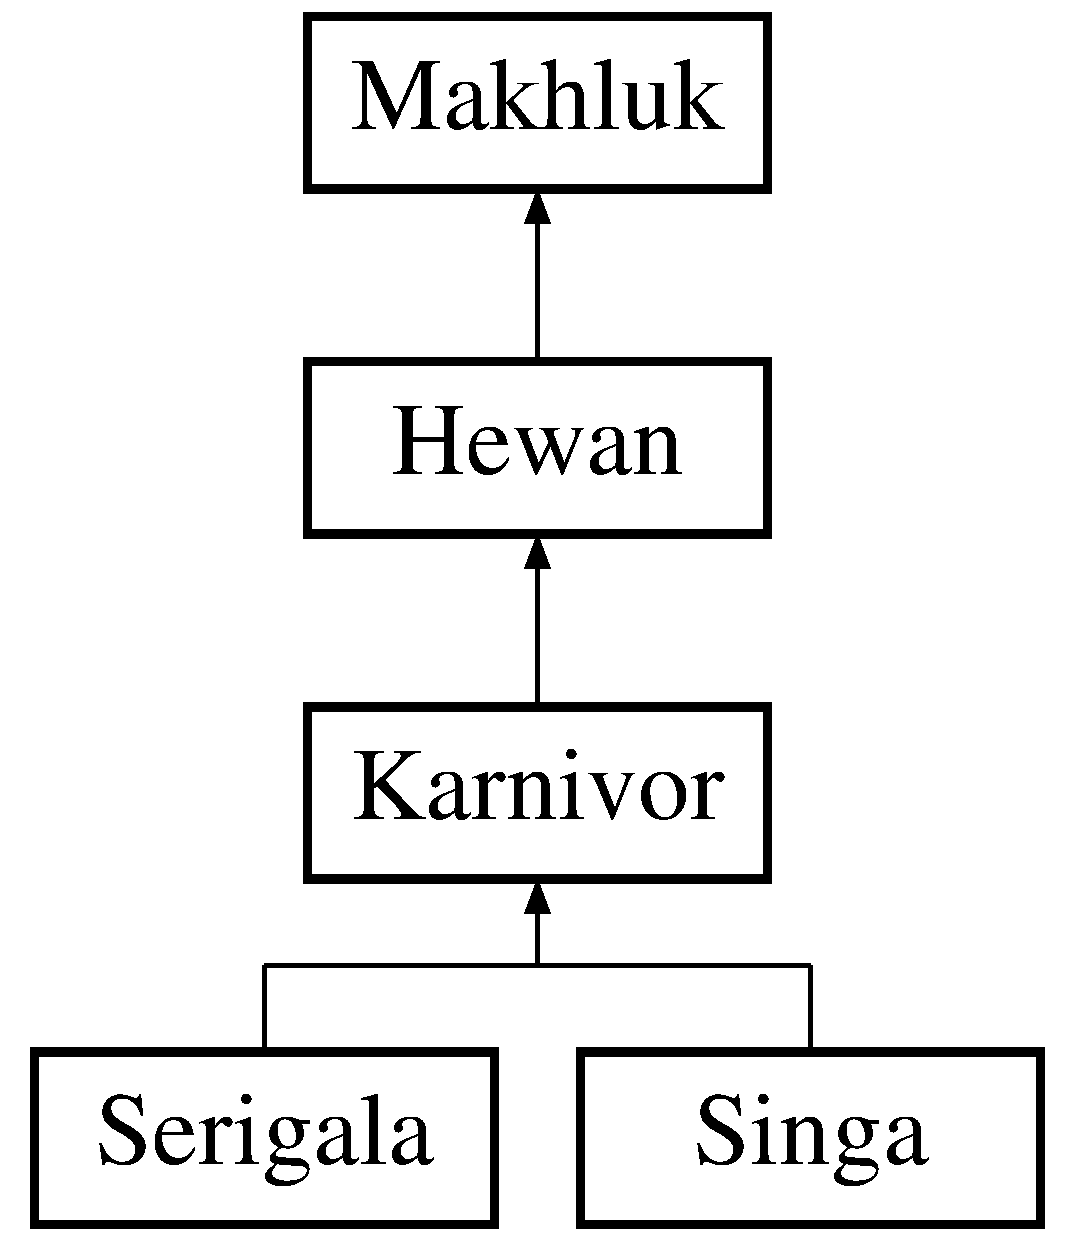
\includegraphics[height=4.000000cm]{class_karnivor}
\end{center}
\end{figure}
\subsection*{Public Member Functions}
\begin{DoxyCompactItemize}
\item 
\hypertarget{class_karnivor_acf8679ded67721322af02c5e2e082562}{}virtual void {\bfseries fight} (\hyperlink{class_karnivor}{Karnivor} $\ast$K)=0\label{class_karnivor_acf8679ded67721322af02c5e2e082562}

\end{DoxyCompactItemize}
\subsection*{Additional Inherited Members}


The documentation for this class was generated from the following file\+:\begin{DoxyCompactItemize}
\item 
src/Karnivor.\+h\end{DoxyCompactItemize}

\hypertarget{class_kuda}{}\section{Kuda Class Reference}
\label{class_kuda}\index{Kuda@{Kuda}}
Inheritance diagram for Kuda\+:\begin{figure}[H]
\begin{center}
\leavevmode
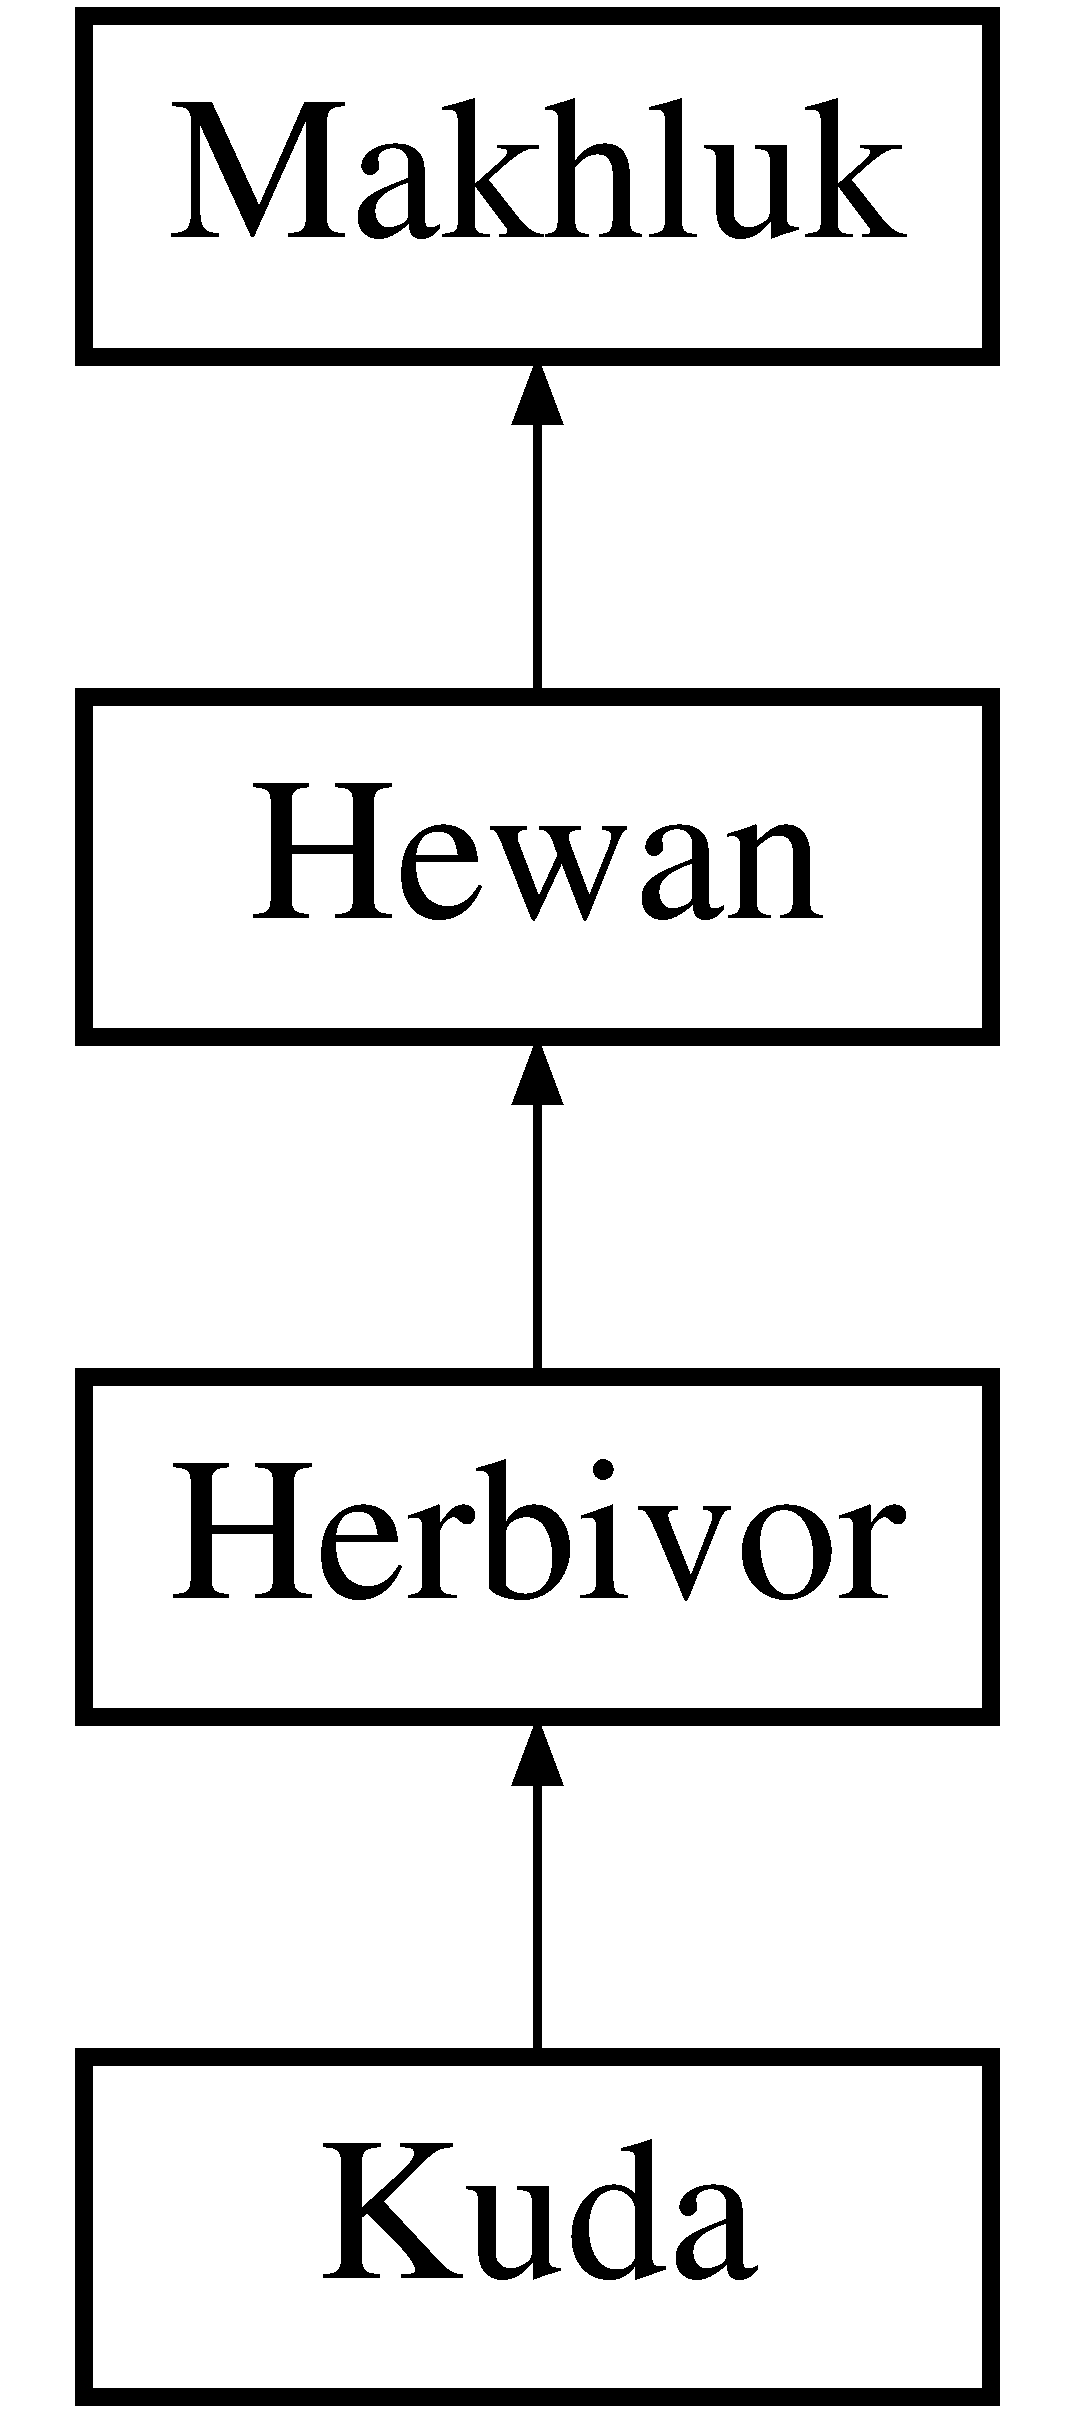
\includegraphics[height=4.000000cm]{class_kuda}
\end{center}
\end{figure}
\subsection*{Public Member Functions}
\begin{DoxyCompactItemize}
\item 
\hypertarget{class_kuda_a35d8c8dc79380dc70ef97d87f7938032}{}{\bfseries Kuda} (int Power, int Usia, int Posisi\+Awal, int Arah\+Gerak, int Id)\label{class_kuda_a35d8c8dc79380dc70ef97d87f7938032}

\item 
\hypertarget{class_kuda_a37132bb9a3e1e6efce091fc16b1191ee}{}void {\bfseries Kill} (int id)\label{class_kuda_a37132bb9a3e1e6efce091fc16b1191ee}

\item 
\hypertarget{class_kuda_ad82609445b57f89833c4d05bab826471}{}void {\bfseries Destruct} ()\label{class_kuda_ad82609445b57f89833c4d05bab826471}

\item 
\hypertarget{class_kuda_a36cd1827c2069b0ee09e086b0442a325}{}void {\bfseries Move} ()\label{class_kuda_a36cd1827c2069b0ee09e086b0442a325}

\item 
\hypertarget{class_kuda_a1d80e3ba3657520926f2a4eb8cb78f02}{}void {\bfseries Pass} ()\label{class_kuda_a1d80e3ba3657520926f2a4eb8cb78f02}

\end{DoxyCompactItemize}
\subsection*{Additional Inherited Members}


The documentation for this class was generated from the following file\+:\begin{DoxyCompactItemize}
\item 
src/Kuda.\+h\end{DoxyCompactItemize}

\hypertarget{class_makhluk}{}\section{Makhluk Class Reference}
\label{class_makhluk}\index{Makhluk@{Makhluk}}
Inheritance diagram for Makhluk\+:\begin{figure}[H]
\begin{center}
\leavevmode
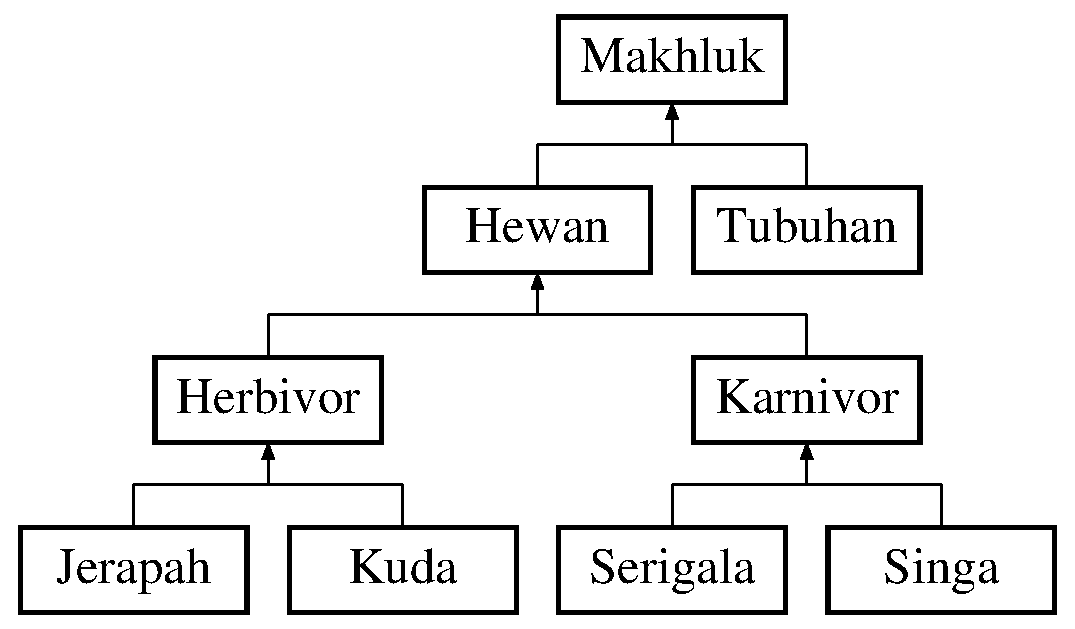
\includegraphics[height=4.000000cm]{class_makhluk}
\end{center}
\end{figure}
\subsection*{Public Member Functions}
\begin{DoxyCompactItemize}
\item 
\hypertarget{class_makhluk_a4c6fd1a0b1f9d0e7cd7e2fb3ecdc8a8a}{}virtual void {\bfseries kill} (int \+\_\+id)=0\label{class_makhluk_a4c6fd1a0b1f9d0e7cd7e2fb3ecdc8a8a}

\item 
\hypertarget{class_makhluk_ac3f695aeecb35405ffdfeb2420a4751d}{}virtual void {\bfseries destruct} ()=0\label{class_makhluk_ac3f695aeecb35405ffdfeb2420a4751d}

\end{DoxyCompactItemize}
\subsection*{Protected Attributes}
\begin{DoxyCompactItemize}
\item 
\hypertarget{class_makhluk_a451e4334ec0ac1a7086a90368f55333a}{}int {\bfseries Power}\label{class_makhluk_a451e4334ec0ac1a7086a90368f55333a}

\item 
\hypertarget{class_makhluk_a4937dd4322359062bb25c67bf8c86d6a}{}int {\bfseries Posisi}\label{class_makhluk_a4937dd4322359062bb25c67bf8c86d6a}

\item 
\hypertarget{class_makhluk_aa7b08651a521198b55ca826da2682aee}{}int {\bfseries Usia}\label{class_makhluk_aa7b08651a521198b55ca826da2682aee}

\end{DoxyCompactItemize}


The documentation for this class was generated from the following file\+:\begin{DoxyCompactItemize}
\item 
src/Makhluk.\+h\end{DoxyCompactItemize}

\hypertarget{class_rumput}{}\section{Rumput Class Reference}
\label{class_rumput}\index{Rumput@{Rumput}}
Inheritance diagram for Rumput\+:\begin{figure}[H]
\begin{center}
\leavevmode
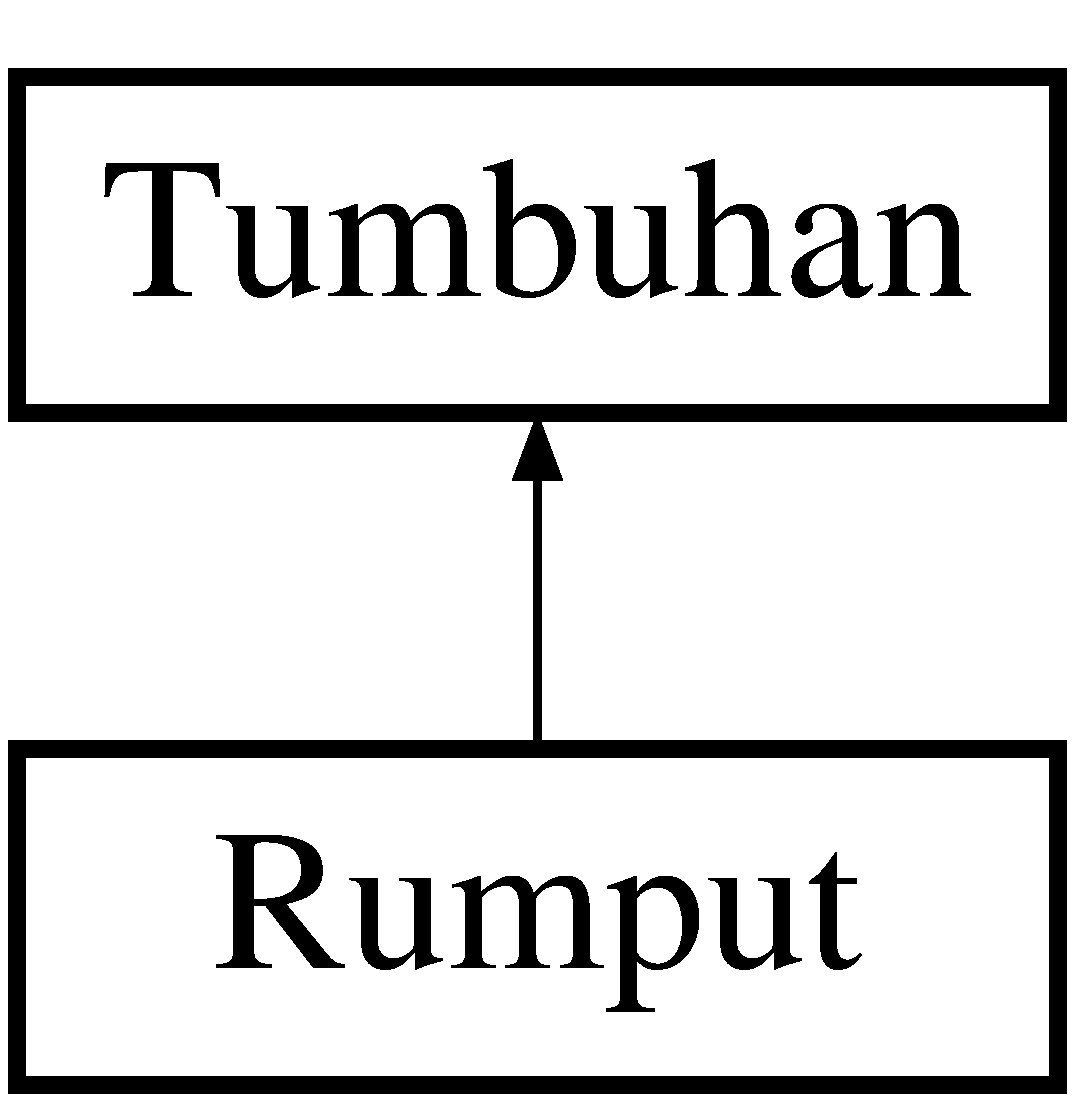
\includegraphics[height=2.000000cm]{class_rumput}
\end{center}
\end{figure}
\subsection*{Public Member Functions}
\begin{DoxyCompactItemize}
\item 
\hypertarget{class_rumput_a8c155d9438a9320ee8b1bc43a34a4c7b}{}{\bfseries Tumbuhan} (int Power, int Usia, int Posisi\+Awal, int Id)\label{class_rumput_a8c155d9438a9320ee8b1bc43a34a4c7b}

\item 
\hypertarget{class_rumput_a3f3f772be251942d9f5c5517d3070e36}{}void {\bfseries Kill} (int id)\label{class_rumput_a3f3f772be251942d9f5c5517d3070e36}

\item 
\hypertarget{class_rumput_ac47b1ece4d9be39237560e8e9ec2ba51}{}void {\bfseries Destruct} ()\label{class_rumput_ac47b1ece4d9be39237560e8e9ec2ba51}

\item 
\hypertarget{class_rumput_aa31831ea757ef45a5c9de5dfd37624cf}{}void {\bfseries Seed} ()\label{class_rumput_aa31831ea757ef45a5c9de5dfd37624cf}

\end{DoxyCompactItemize}


The documentation for this class was generated from the following file\+:\begin{DoxyCompactItemize}
\item 
src/Rumput.\+h\end{DoxyCompactItemize}

\hypertarget{class_serigala}{}\section{Serigala Class Reference}
\label{class_serigala}\index{Serigala@{Serigala}}
Inheritance diagram for Serigala\+:\begin{figure}[H]
\begin{center}
\leavevmode
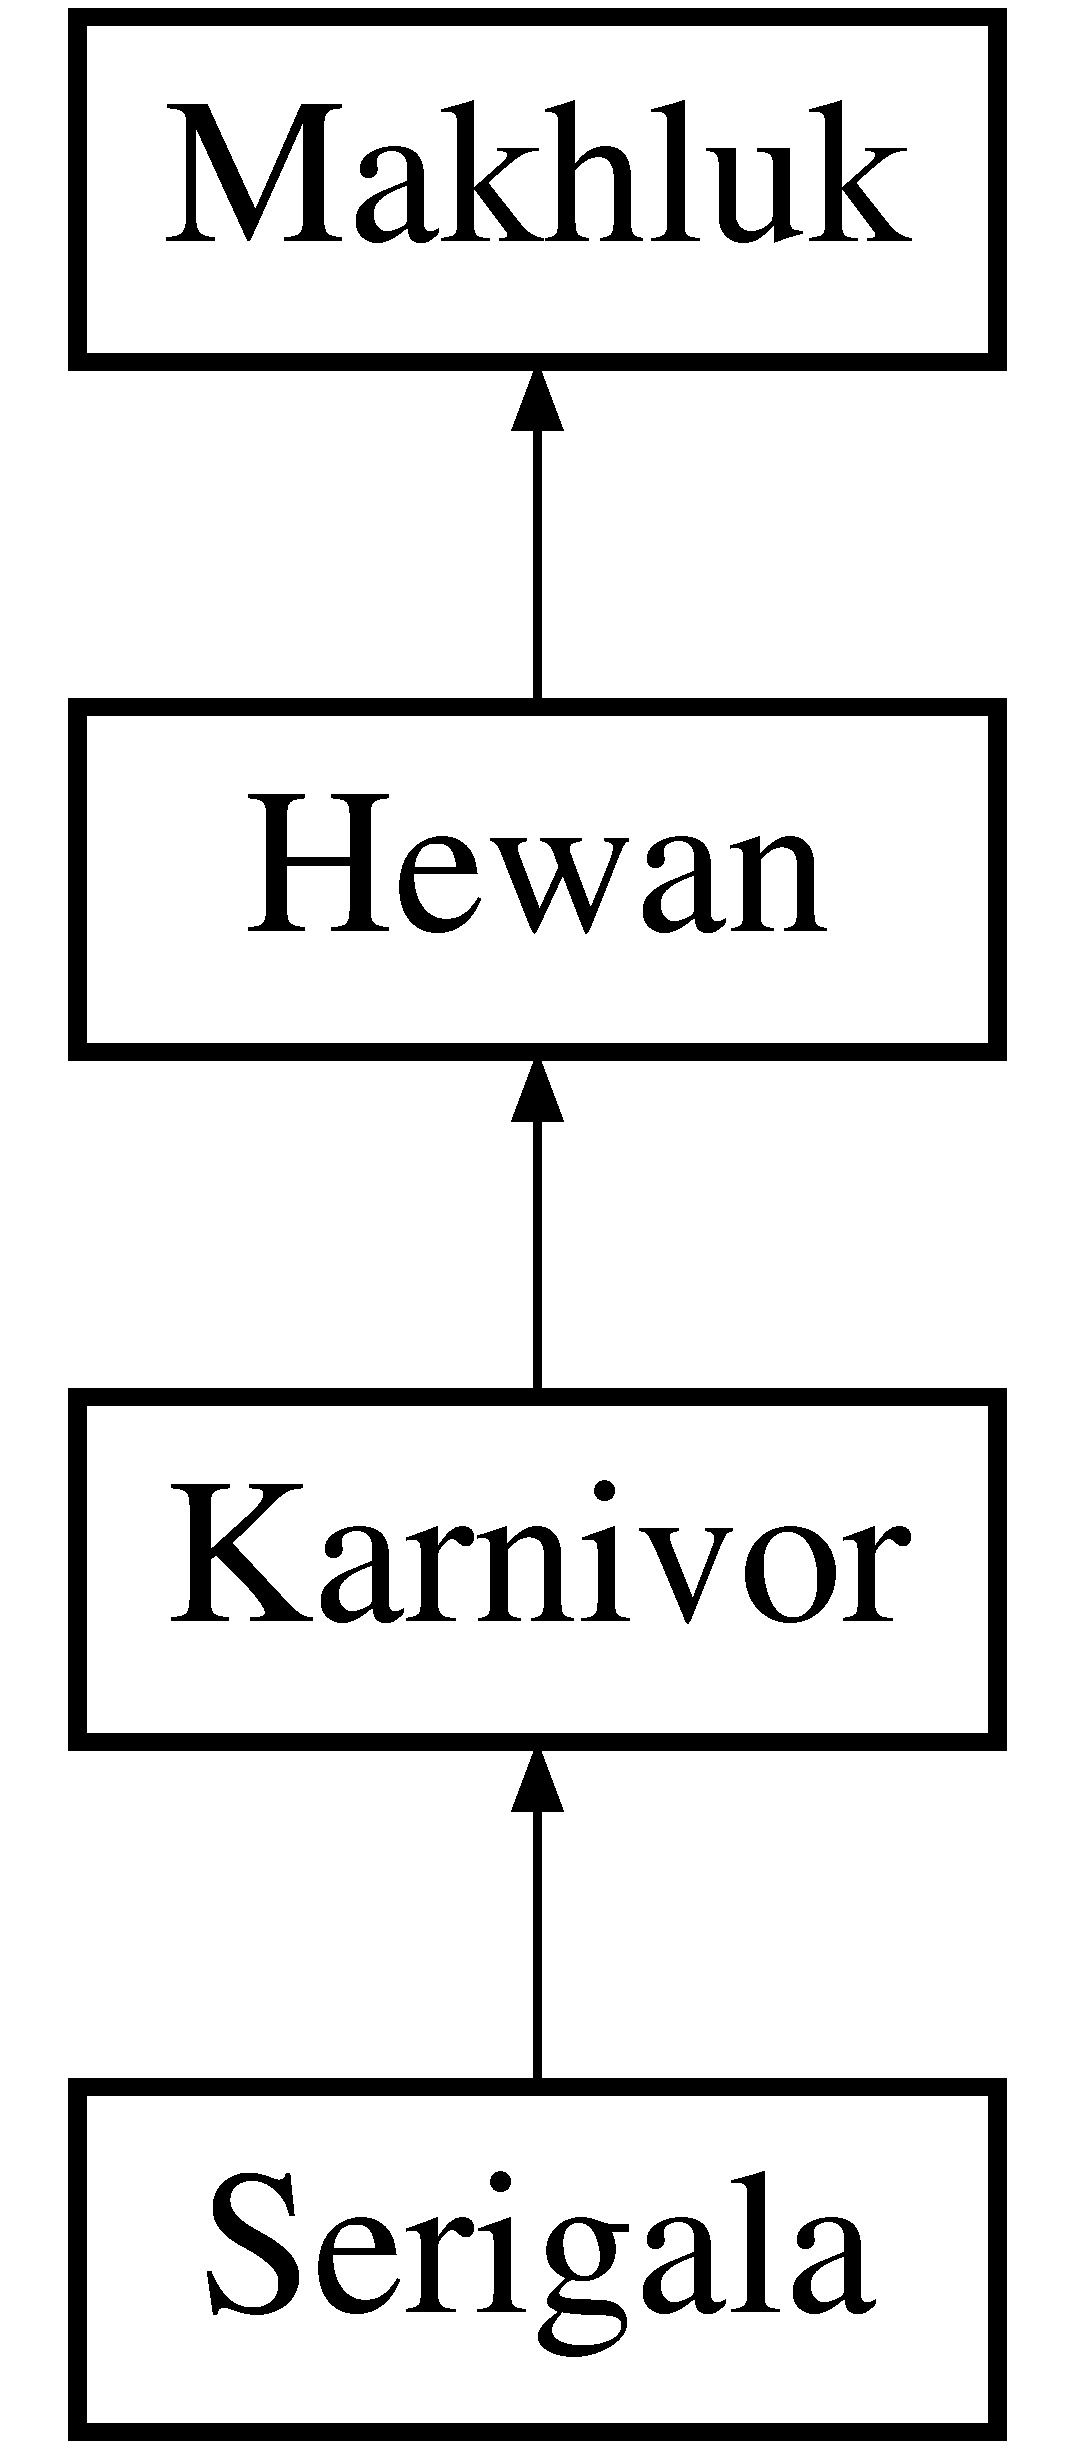
\includegraphics[height=4.000000cm]{class_serigala}
\end{center}
\end{figure}
\subsection*{Public Member Functions}
\begin{DoxyCompactItemize}
\item 
\hypertarget{class_serigala_a2b9182e6082b38f5a345ffc4d0ca6c46}{}{\bfseries Serigala} (int Power, int Usia, int Posisi\+Awal, int Arah\+Gerak, int Id)\label{class_serigala_a2b9182e6082b38f5a345ffc4d0ca6c46}

\item 
\hypertarget{class_serigala_a079dec77b2b1d7988cc7f784e15970b3}{}void {\bfseries Kill} (int id)\label{class_serigala_a079dec77b2b1d7988cc7f784e15970b3}

\item 
\hypertarget{class_serigala_acd1fdf879d7050f699755dd5fc472740}{}void {\bfseries Destruct} ()\label{class_serigala_acd1fdf879d7050f699755dd5fc472740}

\item 
\hypertarget{class_serigala_a39a5f507c9ee63536d1e7ccede8e782f}{}void {\bfseries Move} ()\label{class_serigala_a39a5f507c9ee63536d1e7ccede8e782f}

\item 
\hypertarget{class_serigala_a5c3517dd807a41376731feaa38692ccc}{}void {\bfseries Grouping} ()\label{class_serigala_a5c3517dd807a41376731feaa38692ccc}

\end{DoxyCompactItemize}
\subsection*{Additional Inherited Members}


The documentation for this class was generated from the following file\+:\begin{DoxyCompactItemize}
\item 
src/Serigala.\+h\end{DoxyCompactItemize}

\hypertarget{class_singa}{}\section{Singa Class Reference}
\label{class_singa}\index{Singa@{Singa}}


{\ttfamily \#include $<$Singa.\+h$>$}

Inheritance diagram for Singa\+:\begin{figure}[H]
\begin{center}
\leavevmode
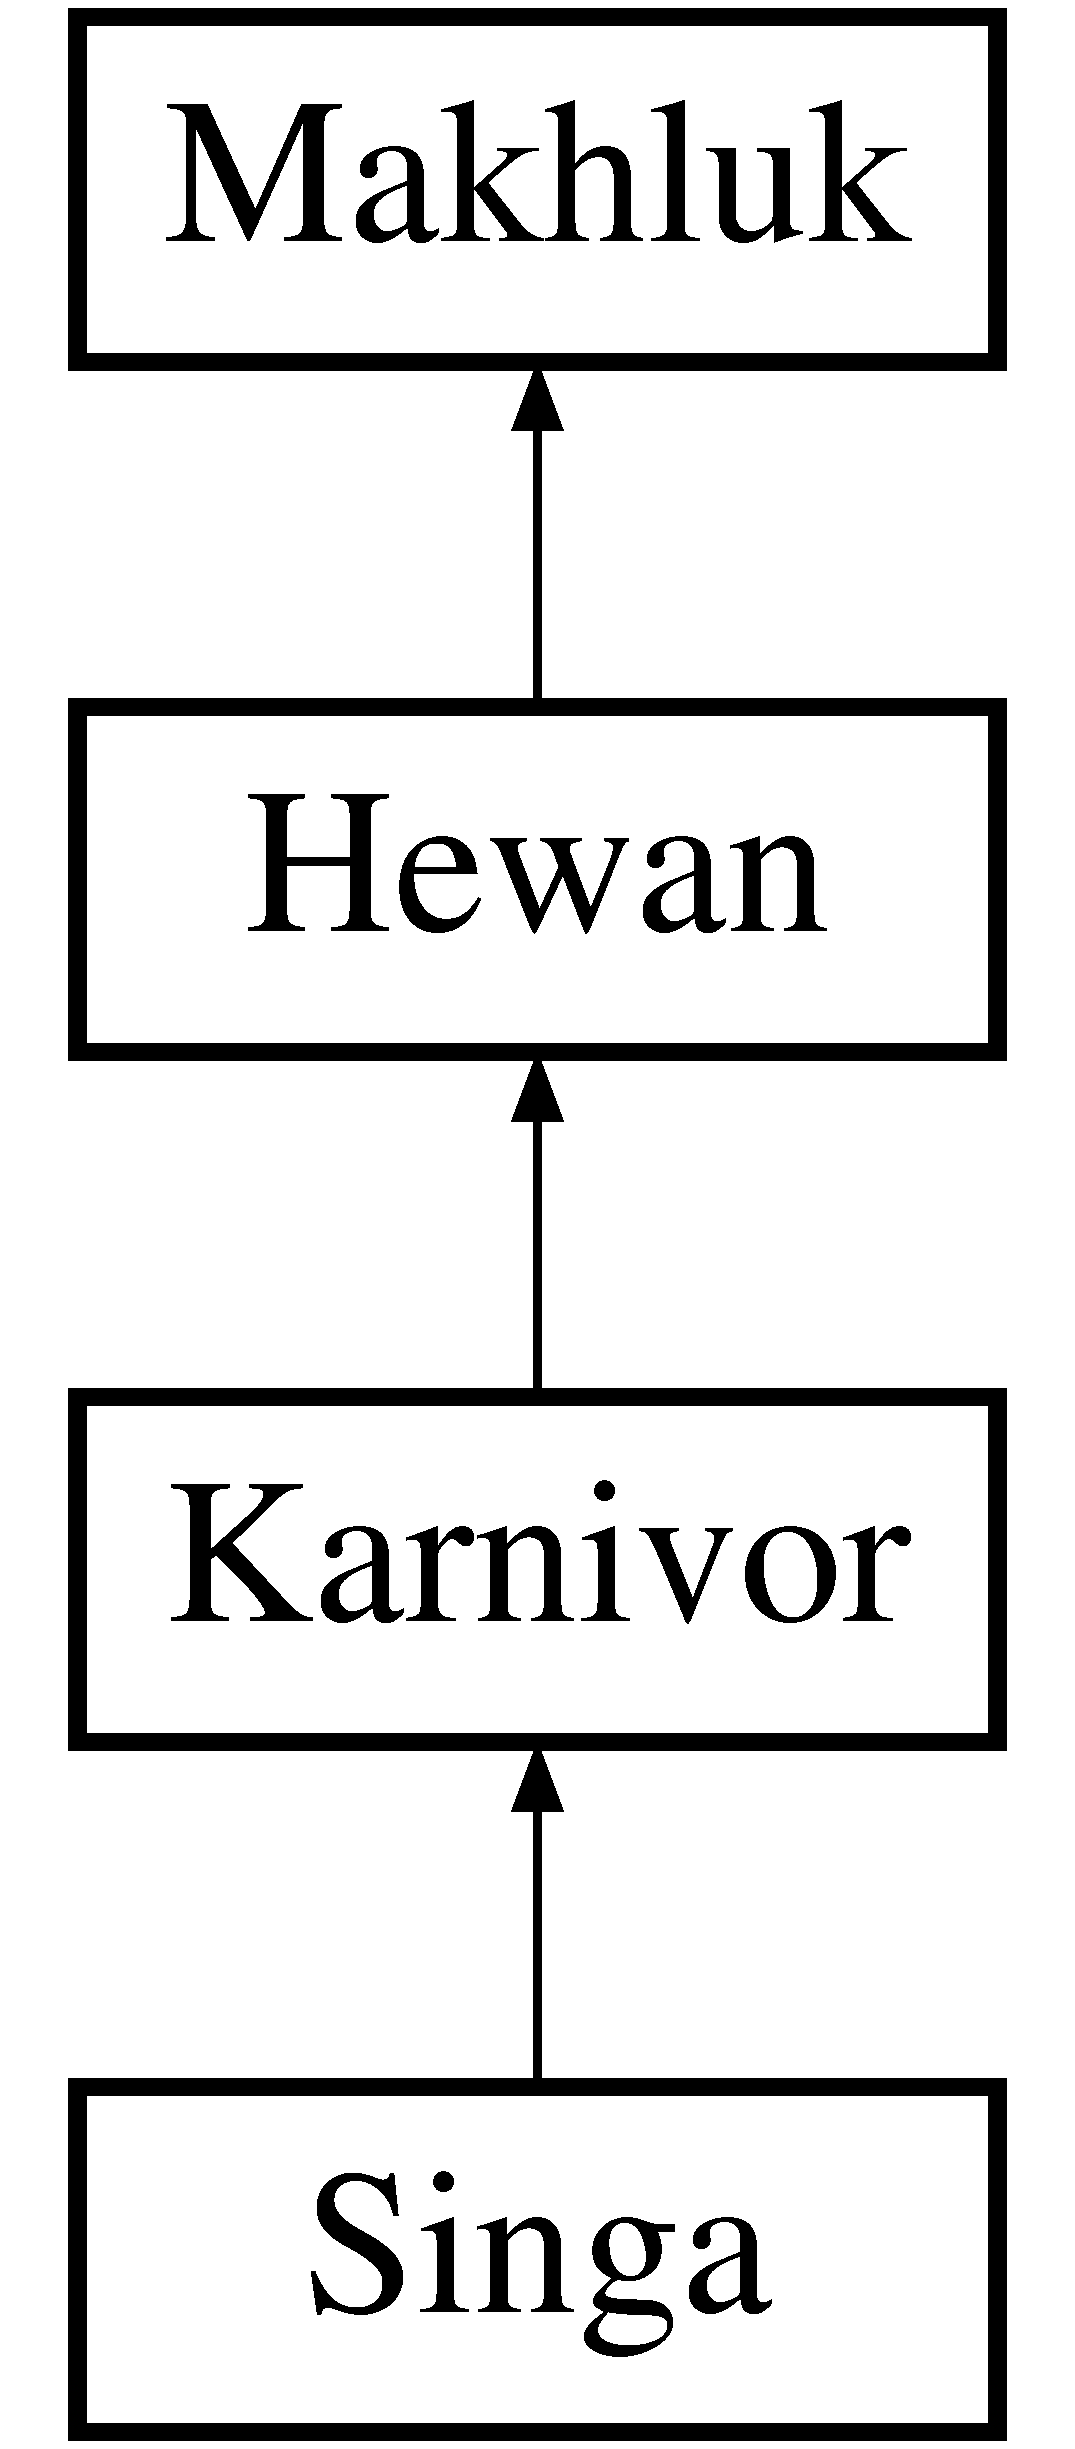
\includegraphics[height=4.000000cm]{class_singa}
\end{center}
\end{figure}
\subsection*{Public Member Functions}
\begin{DoxyCompactItemize}
\item 
\hyperlink{class_singa_a2b6bc8f6bd4293c487734b5663b598ce}{Singa} ()
\item 
\hyperlink{class_singa_ad7b8861fb589c68e6a88f7295dc05fc1}{Singa} (int \+\_\+\+Power, int \+\_\+\+Usia, int \+\_\+\+Posisi, int \+\_\+\+Arah\+Gerak, int \+\_\+\+Id)
\item 
\hyperlink{class_singa_a4b2f9063d9d97cbf41f05c3558b2b9a6}{$\sim$\+Singa} ()
\item 
int \hyperlink{class_singa_aef63a0687ca6369e48130423ecfa6187}{Get\+Id} ()
\item 
int \hyperlink{class_singa_a915a753437feec3e980c1a8b57b301d7}{Get\+Usia} ()
\item 
int \hyperlink{class_singa_a54f4006c51cf3f8f0f8eb733768a08d8}{Get\+Posisi} ()
\item 
int \hyperlink{class_singa_a12c8893d99f2a8b080cc4549c2db193d}{Get\+Arah\+Gerak} ()
\item 
void \hyperlink{class_singa_a9ac8600a62bc6f33a42bfc2cd4d5d426}{Set\+Arah\+Gerak} (int \+\_\+\+Arah\+Gerak)
\item 
void \hyperlink{class_singa_adfcf66d135f5dc72060400e74173aa76}{Set\+Posisi} (int \+\_\+\+Posisi)
\item 
void \hyperlink{class_singa_a65ea5d6280ff39f313b5829130b7bcf8}{Set\+Usia} (int \+\_\+usia)
\item 
\hypertarget{class_singa_ab8af9a6523f0fe43eb04f1240c4f0804}{}void {\bfseries kill} (int \+\_\+id)\label{class_singa_ab8af9a6523f0fe43eb04f1240c4f0804}

\item 
void \hyperlink{class_singa_acdcf6232b3a5c17b85fddbac64d7f3f0}{destruct} ()
\item 
void \hyperlink{class_singa_ab4a3ab4c47f2635944e2ac4a58953377}{move} ()
\item 
void \hyperlink{class_singa_aaf195d0fe8ca4755edcc0fc6e168cbb5}{grouping} ()
\item 
void \hyperlink{class_singa_a78556ed2114916e5b00234ef931b0e58}{fight} (\hyperlink{class_karnivor}{Karnivor} $\ast$K)
\end{DoxyCompactItemize}
\subsection*{Additional Inherited Members}


\subsection{Detailed Description}
Kelas yang merepresantikan singa dan beberapa sifatnya 

\subsection{Constructor \& Destructor Documentation}
\hypertarget{class_singa_a2b6bc8f6bd4293c487734b5663b598ce}{}\index{Singa@{Singa}!Singa@{Singa}}
\index{Singa@{Singa}!Singa@{Singa}}
\subsubsection[{Singa}]{\setlength{\rightskip}{0pt plus 5cm}Singa\+::\+Singa (
\begin{DoxyParamCaption}
{}
\end{DoxyParamCaption}
)}\label{class_singa_a2b6bc8f6bd4293c487734b5663b598ce}
Public Method that implement virtual function from parents class \hypertarget{class_singa_ad7b8861fb589c68e6a88f7295dc05fc1}{}\index{Singa@{Singa}!Singa@{Singa}}
\index{Singa@{Singa}!Singa@{Singa}}
\subsubsection[{Singa}]{\setlength{\rightskip}{0pt plus 5cm}Singa\+::\+Singa (
\begin{DoxyParamCaption}
\item[{int}]{\+\_\+\+Power, }
\item[{int}]{\+\_\+\+Usia, }
\item[{int}]{\+\_\+\+Posisi, }
\item[{int}]{\+\_\+\+Arah\+Gerak, }
\item[{int}]{\+\_\+\+Id}
\end{DoxyParamCaption}
)}\label{class_singa_ad7b8861fb589c68e6a88f7295dc05fc1}
Standard constructor, give default value of power, usia, posisi, arahgerak, id \hypertarget{class_singa_a4b2f9063d9d97cbf41f05c3558b2b9a6}{}\index{Singa@{Singa}!````~Singa@{$\sim$\+Singa}}
\index{````~Singa@{$\sim$\+Singa}!Singa@{Singa}}
\subsubsection[{$\sim$\+Singa}]{\setlength{\rightskip}{0pt plus 5cm}Singa\+::$\sim$\+Singa (
\begin{DoxyParamCaption}
{}
\end{DoxyParamCaption}
)}\label{class_singa_a4b2f9063d9d97cbf41f05c3558b2b9a6}
Params constructor where you have to give all the parameter manually 

\subsection{Member Function Documentation}
\hypertarget{class_singa_acdcf6232b3a5c17b85fddbac64d7f3f0}{}\index{Singa@{Singa}!destruct@{destruct}}
\index{destruct@{destruct}!Singa@{Singa}}
\subsubsection[{destruct}]{\setlength{\rightskip}{0pt plus 5cm}void Singa\+::destruct (
\begin{DoxyParamCaption}
{}
\end{DoxyParamCaption}
)\hspace{0.3cm}{\ttfamily [virtual]}}\label{class_singa_acdcf6232b3a5c17b85fddbac64d7f3f0}
Kill other creature, invoke other creature \hyperlink{class_singa_acdcf6232b3a5c17b85fddbac64d7f3f0}{destruct()} 

Implements \hyperlink{class_makhluk}{Makhluk}.

\hypertarget{class_singa_a78556ed2114916e5b00234ef931b0e58}{}\index{Singa@{Singa}!fight@{fight}}
\index{fight@{fight}!Singa@{Singa}}
\subsubsection[{fight}]{\setlength{\rightskip}{0pt plus 5cm}void Singa\+::fight (
\begin{DoxyParamCaption}
\item[{{\bf Karnivor} $\ast$}]{K}
\end{DoxyParamCaption}
)\hspace{0.3cm}{\ttfamily [virtual]}}\label{class_singa_a78556ed2114916e5b00234ef931b0e58}
When singa meet other singa, they\textquotesingle{}ll form a group 

Implements \hyperlink{class_karnivor}{Karnivor}.

\hypertarget{class_singa_a12c8893d99f2a8b080cc4549c2db193d}{}\index{Singa@{Singa}!Get\+Arah\+Gerak@{Get\+Arah\+Gerak}}
\index{Get\+Arah\+Gerak@{Get\+Arah\+Gerak}!Singa@{Singa}}
\subsubsection[{Get\+Arah\+Gerak}]{\setlength{\rightskip}{0pt plus 5cm}int Singa\+::\+Get\+Arah\+Gerak (
\begin{DoxyParamCaption}
{}
\end{DoxyParamCaption}
)}\label{class_singa_a12c8893d99f2a8b080cc4549c2db193d}
Return Posisi of singa \hypertarget{class_singa_aef63a0687ca6369e48130423ecfa6187}{}\index{Singa@{Singa}!Get\+Id@{Get\+Id}}
\index{Get\+Id@{Get\+Id}!Singa@{Singa}}
\subsubsection[{Get\+Id}]{\setlength{\rightskip}{0pt plus 5cm}int Singa\+::\+Get\+Id (
\begin{DoxyParamCaption}
{}
\end{DoxyParamCaption}
)}\label{class_singa_aef63a0687ca6369e48130423ecfa6187}
destructor, no delete\mbox{[}\mbox{]} because there\textquotesingle{}s no pointer data. \hypertarget{class_singa_a54f4006c51cf3f8f0f8eb733768a08d8}{}\index{Singa@{Singa}!Get\+Posisi@{Get\+Posisi}}
\index{Get\+Posisi@{Get\+Posisi}!Singa@{Singa}}
\subsubsection[{Get\+Posisi}]{\setlength{\rightskip}{0pt plus 5cm}int Singa\+::\+Get\+Posisi (
\begin{DoxyParamCaption}
{}
\end{DoxyParamCaption}
)}\label{class_singa_a54f4006c51cf3f8f0f8eb733768a08d8}
Return Usia of singa \hypertarget{class_singa_a915a753437feec3e980c1a8b57b301d7}{}\index{Singa@{Singa}!Get\+Usia@{Get\+Usia}}
\index{Get\+Usia@{Get\+Usia}!Singa@{Singa}}
\subsubsection[{Get\+Usia}]{\setlength{\rightskip}{0pt plus 5cm}int Singa\+::\+Get\+Usia (
\begin{DoxyParamCaption}
{}
\end{DoxyParamCaption}
)}\label{class_singa_a915a753437feec3e980c1a8b57b301d7}
Return Id of a \hyperlink{class_singa}{Singa} \hypertarget{class_singa_aaf195d0fe8ca4755edcc0fc6e168cbb5}{}\index{Singa@{Singa}!grouping@{grouping}}
\index{grouping@{grouping}!Singa@{Singa}}
\subsubsection[{grouping}]{\setlength{\rightskip}{0pt plus 5cm}void Singa\+::grouping (
\begin{DoxyParamCaption}
{}
\end{DoxyParamCaption}
)\hspace{0.3cm}{\ttfamily [virtual]}}\label{class_singa_aaf195d0fe8ca4755edcc0fc6e168cbb5}
Move the \hyperlink{class_singa}{Singa} 

Implements \hyperlink{class_hewan}{Hewan}.

\hypertarget{class_singa_ab4a3ab4c47f2635944e2ac4a58953377}{}\index{Singa@{Singa}!move@{move}}
\index{move@{move}!Singa@{Singa}}
\subsubsection[{move}]{\setlength{\rightskip}{0pt plus 5cm}void Singa\+::move (
\begin{DoxyParamCaption}
{}
\end{DoxyParamCaption}
)\hspace{0.3cm}{\ttfamily [virtual]}}\label{class_singa_ab4a3ab4c47f2635944e2ac4a58953377}
Destruct because death by age or killed by other creature 

Implements \hyperlink{class_hewan}{Hewan}.

\hypertarget{class_singa_a9ac8600a62bc6f33a42bfc2cd4d5d426}{}\index{Singa@{Singa}!Set\+Arah\+Gerak@{Set\+Arah\+Gerak}}
\index{Set\+Arah\+Gerak@{Set\+Arah\+Gerak}!Singa@{Singa}}
\subsubsection[{Set\+Arah\+Gerak}]{\setlength{\rightskip}{0pt plus 5cm}void Singa\+::\+Set\+Arah\+Gerak (
\begin{DoxyParamCaption}
\item[{int}]{\+\_\+\+Arah\+Gerak}
\end{DoxyParamCaption}
)}\label{class_singa_a9ac8600a62bc6f33a42bfc2cd4d5d426}
Return Arah\+Gerak of singa \hypertarget{class_singa_adfcf66d135f5dc72060400e74173aa76}{}\index{Singa@{Singa}!Set\+Posisi@{Set\+Posisi}}
\index{Set\+Posisi@{Set\+Posisi}!Singa@{Singa}}
\subsubsection[{Set\+Posisi}]{\setlength{\rightskip}{0pt plus 5cm}void Singa\+::\+Set\+Posisi (
\begin{DoxyParamCaption}
\item[{int}]{\+\_\+\+Posisi}
\end{DoxyParamCaption}
)}\label{class_singa_adfcf66d135f5dc72060400e74173aa76}
change Arah\+Gerak, will be useful for \hyperlink{class_singa_a78556ed2114916e5b00234ef931b0e58}{fight()} function \hypertarget{class_singa_a65ea5d6280ff39f313b5829130b7bcf8}{}\index{Singa@{Singa}!Set\+Usia@{Set\+Usia}}
\index{Set\+Usia@{Set\+Usia}!Singa@{Singa}}
\subsubsection[{Set\+Usia}]{\setlength{\rightskip}{0pt plus 5cm}void Singa\+::\+Set\+Usia (
\begin{DoxyParamCaption}
\item[{int}]{\+\_\+usia}
\end{DoxyParamCaption}
)}\label{class_singa_a65ea5d6280ff39f313b5829130b7bcf8}
Set Posisi of singa 

The documentation for this class was generated from the following files\+:\begin{DoxyCompactItemize}
\item 
src/Singa.\+h\item 
src/Singa.\+cpp\end{DoxyCompactItemize}

\hypertarget{class_tubuhan}{}\section{Tubuhan Class Reference}
\label{class_tubuhan}\index{Tubuhan@{Tubuhan}}
Inheritance diagram for Tubuhan\+:\begin{figure}[H]
\begin{center}
\leavevmode
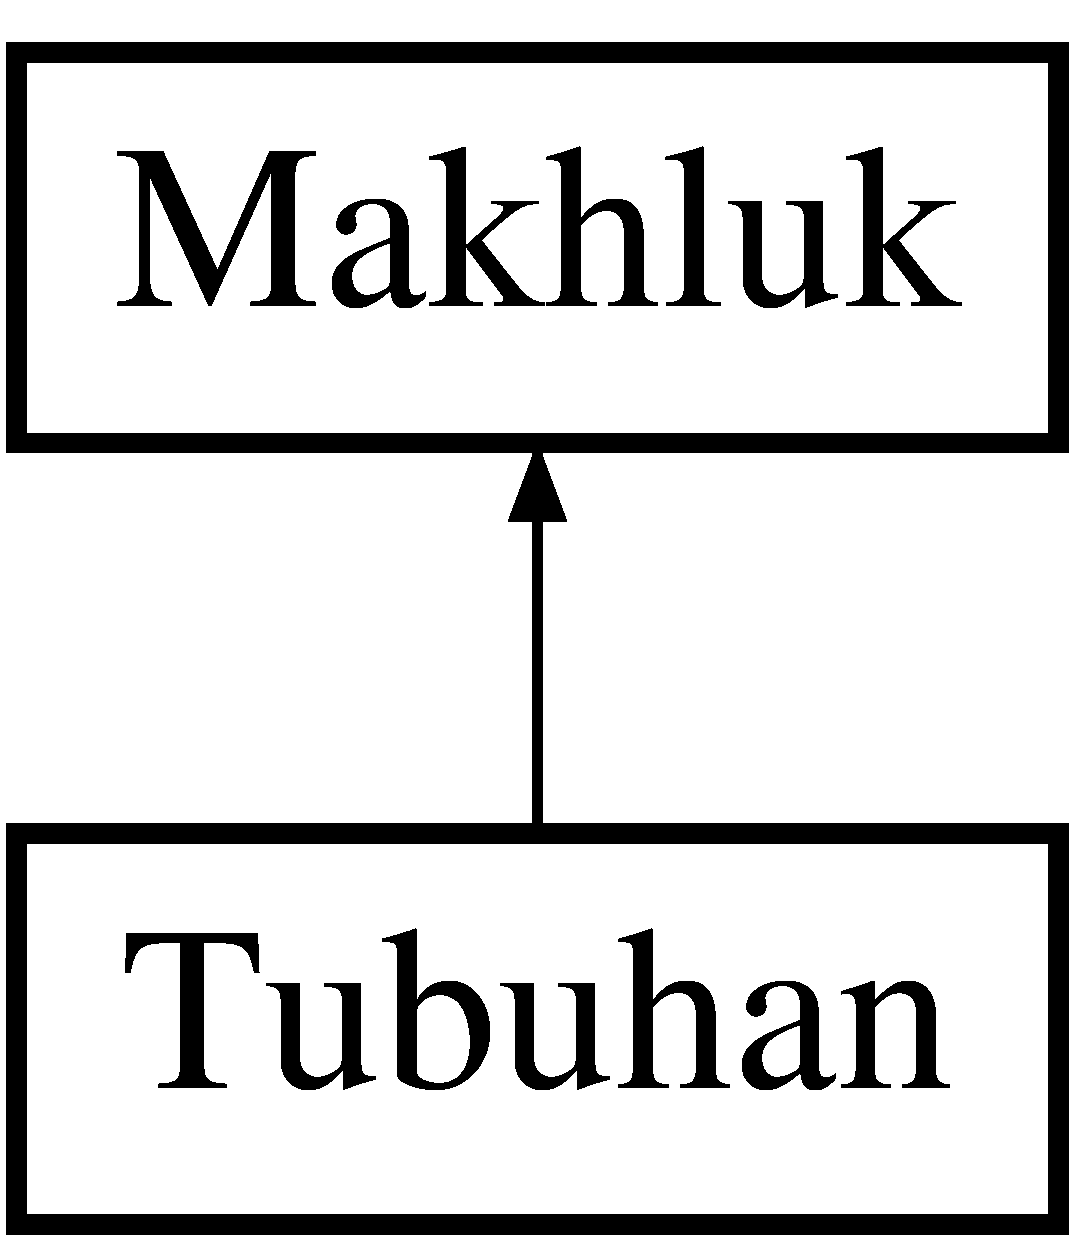
\includegraphics[height=2.000000cm]{class_tubuhan}
\end{center}
\end{figure}
\subsection*{Public Member Functions}
\begin{DoxyCompactItemize}
\item 
\hypertarget{class_tubuhan_a499f3dc22b711bb42d60744ec649310d}{}virtual void {\bfseries Seed} ()=0\label{class_tubuhan_a499f3dc22b711bb42d60744ec649310d}

\end{DoxyCompactItemize}
\subsection*{Additional Inherited Members}


The documentation for this class was generated from the following file\+:\begin{DoxyCompactItemize}
\item 
src/Tumbuhan.\+h\end{DoxyCompactItemize}

\hypertarget{class_wortel}{}\section{Wortel Class Reference}
\label{class_wortel}\index{Wortel@{Wortel}}
Inheritance diagram for Wortel\+:\begin{figure}[H]
\begin{center}
\leavevmode
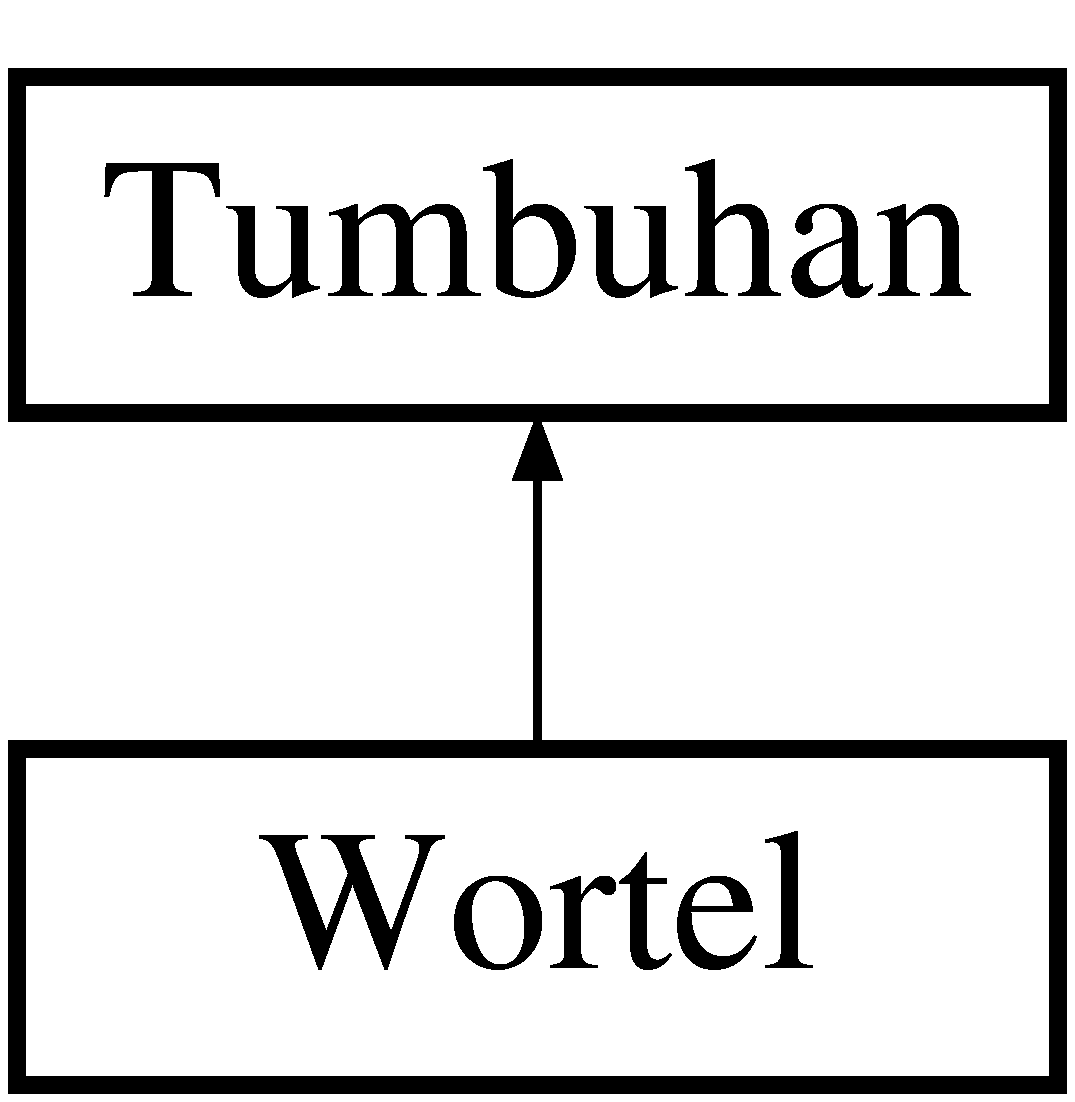
\includegraphics[height=2.000000cm]{class_wortel}
\end{center}
\end{figure}
\subsection*{Public Member Functions}
\begin{DoxyCompactItemize}
\item 
\hypertarget{class_wortel_a5cacd30f4c7133c7a9c657da54f88d16}{}{\bfseries Wortel} (int Power, int Usia, int Posisi\+Awal, int Id)\label{class_wortel_a5cacd30f4c7133c7a9c657da54f88d16}

\item 
\hypertarget{class_wortel_af7a79a9e1b4d15bd3f7498beb0ea8be1}{}void {\bfseries Kill} (int id)\label{class_wortel_af7a79a9e1b4d15bd3f7498beb0ea8be1}

\item 
\hypertarget{class_wortel_a520a82f28b6c65b98605d051768e88b7}{}void {\bfseries Destruct} ()\label{class_wortel_a520a82f28b6c65b98605d051768e88b7}

\item 
\hypertarget{class_wortel_aa5acbe42d876893154b87c924e4e02a4}{}void {\bfseries Seed} ()\label{class_wortel_aa5acbe42d876893154b87c924e4e02a4}

\end{DoxyCompactItemize}


The documentation for this class was generated from the following file\+:\begin{DoxyCompactItemize}
\item 
src/Wortel.\+h\end{DoxyCompactItemize}

%--- End generated contents ---

% Index
\backmatter
\newpage
\phantomsection
\clearemptydoublepage
\addcontentsline{toc}{chapter}{Index}
\printindex

\end{document}
